\documentclass[12pt,a4paper]{article}
\pdfoutput=1
%vons grund
\usepackage[utf8]{inputenc}
\usepackage[T1]{fontenc}
\usepackage[swedish]{babel} %OBS! Se till att vi får rätt språk.
\usepackage{amsmath}
\usepackage{lmodern}
\usepackage{units}
\usepackage{icomma}
\usepackage{color}
\usepackage{graphicx}
\usepackage{bbm}
\newcommand{\N}{\ensuremath{\mathbbm{N}}}
\newcommand{\Z}{\ensuremath{\mathbbm{Z}}}
\newcommand{\Q}{\ensuremath{\mathbbm{Q}}}
\newcommand{\R}{\ensuremath{\mathbbm{R}}}
\newcommand{\C}{\ensuremath{\mathbbm{C}}}
\newcommand{\rd}{\ensuremath{\mathrm{d}}}
\newcommand{\id}{\ensuremath{\,\rd}}
\usepackage{hyperref}

%%%%%%%%%%%%%%%%%%%%%%%Egna tillägg%%%%%%%%%%%%%%%%%%%%%%%

%%Partiell derivata
\newcommand{\pd}{\ensuremath{\partial}}
%%Följer ISO-8601 oberoende av språk.
\usepackage{datetime} 
\newdateformat{specialdate}{\THEYEAR-\twodigit{\THEMONTH}-\twodigit{\THEDAY}}
%%Göra grader Celcius
\newcommand{\degC}{\ensuremath{\,^\circ\mathrm{C}}}
%%Figurreferenser
\newcommand{\Figref}{\figurename~\ref} %Stor bokstav i början
\newcommand{\figref}{\MakeLowercase{\figurename}~\ref} 
%%Tabellreferenser
\newcommand{\Tabref}{\tablename~\ref} %Stor bokstav i början
\newcommand{\tabref}{\MakeLowercase{\tablename}~\ref}
%%Ohm enhetskommando
\newcommand{\ohm}{\ifmmode \Omega \else $\Omega$ \fi}
%%Varepsilon är det enda rätta epsilon
\renewcommand{\epsilon}{\varepsilon}


%%%%%%%%%%%%%%%%%%Övriga matnyttiga paket%%%%%%%%%%%%%%%%%

%%För att kunna inkludera andra PDF-dokument
\usepackage{pdfpages}
%%För att kunna ha roterade bilder
\usepackage{rotating}
%%För att inkludera MATLABkod. 
%\usepackage[framed,numbered,autolinebreaks,useliterate]{mcode}
%\usepackage{listings} 
%\lstloadlanguages{matlab} 
%\lstset{language=matlab} 
%\lstset{literate= {å}{{\r{a}}}1 {ä}{{\"a}}1 {ö}{{\"o}}1 {Å}{{\r{A}}}1
%  {Ä}{{\"A}}1 {Ö}{{\"O}}1}%För att få svenska bokstäver från MATLAB.


%%För att själv bestämma marginalerna. 
%\usepackage[
%            top    = 3cm,
%            bottom = 3cm,
%            left   = 3cm, right  = 3cm
%]{geometry}


\usepackage{sectsty}
\sectionfont{\fontsize{13}{0}\selectfont}



\begin{document}
\title{LED-karakteristik}
\author{}
\date{}
\maketitle


% \section*{Bakgrund} 
% Nobelpriset i fysik 2014 gavs till Isamu Akasaki, Hiroshi Amano och
% Shuji Nakamura för deras genombrott med blåa LED:er (Light Emitting
% Diode). Med blåa LED:er blev det plötsligt möjligt att skapa en
% ''vit'' lysdiod. Genom att kombinera röda, gröna och blåa LED:er kan
% man skapa en lysdiod som ser ut att lysa vitt för ögat (jämför en dators
% bildskärm: RGB).

%\section*{Uppgift}
När man ska konstruera en ''vit'' lysdiod kan man ''parallellkoppla''
LED:er av respektive färg. Man måste dock först seriekoppla varje LED
med en resistor innan man kan ''parallellkoppla'' dem, ungefär som i
\figref{svart_låda}.  

\begin{enumerate}
\item Mät upp karakteristiken (ström som funktion av
spänning) för en röd respektive blå LED. Svara med grafer för
respektive LED (kan göras på samma diagram/papper, men du måste
tydligt markera vliken graf som hör till vilken LED).
\item Argumentera utifrån din uppmätta karakteristik vad som skulle
  hända om du försökte parallellkoppla två olika LED:er utan något
  seriemotstånd? 
\end{enumerate}
Till ditt förfogande finns en
''svart låda'' (öppna inte!) med en blå och en röd LED som sticker ut. 
Glöm inte att rita ditt kopplingsschema där även alla mätinstrument
finns med!

\emph{Tips}: En äkta parallellkoppling kännetäcknas av att samma
spänning ligger över båda två av de parallellkopplade komponenterna. 

%föreslå serieresistanser, $R_1$ och $R_2$ enligt
%\figref{parallell},  
%så att en lika stor ström, $i=\unit[5]{mA}$, flyter genom både den
%röda och den blå LED:en om en spänning, $E=\unit[5]{V}$ kopplas in
%i \figref{parallell}. 


% \begin{figure}\centering
% \input{parallell.pdf_t}
% \caption{\label{parallell} En röd och en blå LED ''parallellkopplade''
% med respektive seriemotstånd, $R_1$ och $R_2$ (detta är alltså
% separata komponenter och är inte del av själva LED:erna).}
% \end{figure}



%\newpage
\section*{Materiel}

\begin{itemize}
\item 1 ''Svart låda'' som är kontruerad enligt \figref{svart_låda}.
\item 2 Multimetrar
\item 5 Labbsladdar
\item Milimeterpapper
\end{itemize}


\begin{figure}\centering
\input{svart_lada.pdf_t}
\caption{\label{svart_låda} ''Svart låda''. Du kommer att ha tillgång
  till de två polerna utanför lådan och strömbrytaren för att koppla in den
  blå lysdioden. Du kommer även att kunna se LED:erna för att
  kontrollera ifall de lyser eller inte. }
\end{figure}

\begin{figure}\centering
\centerline{ %centrerar även större bilder
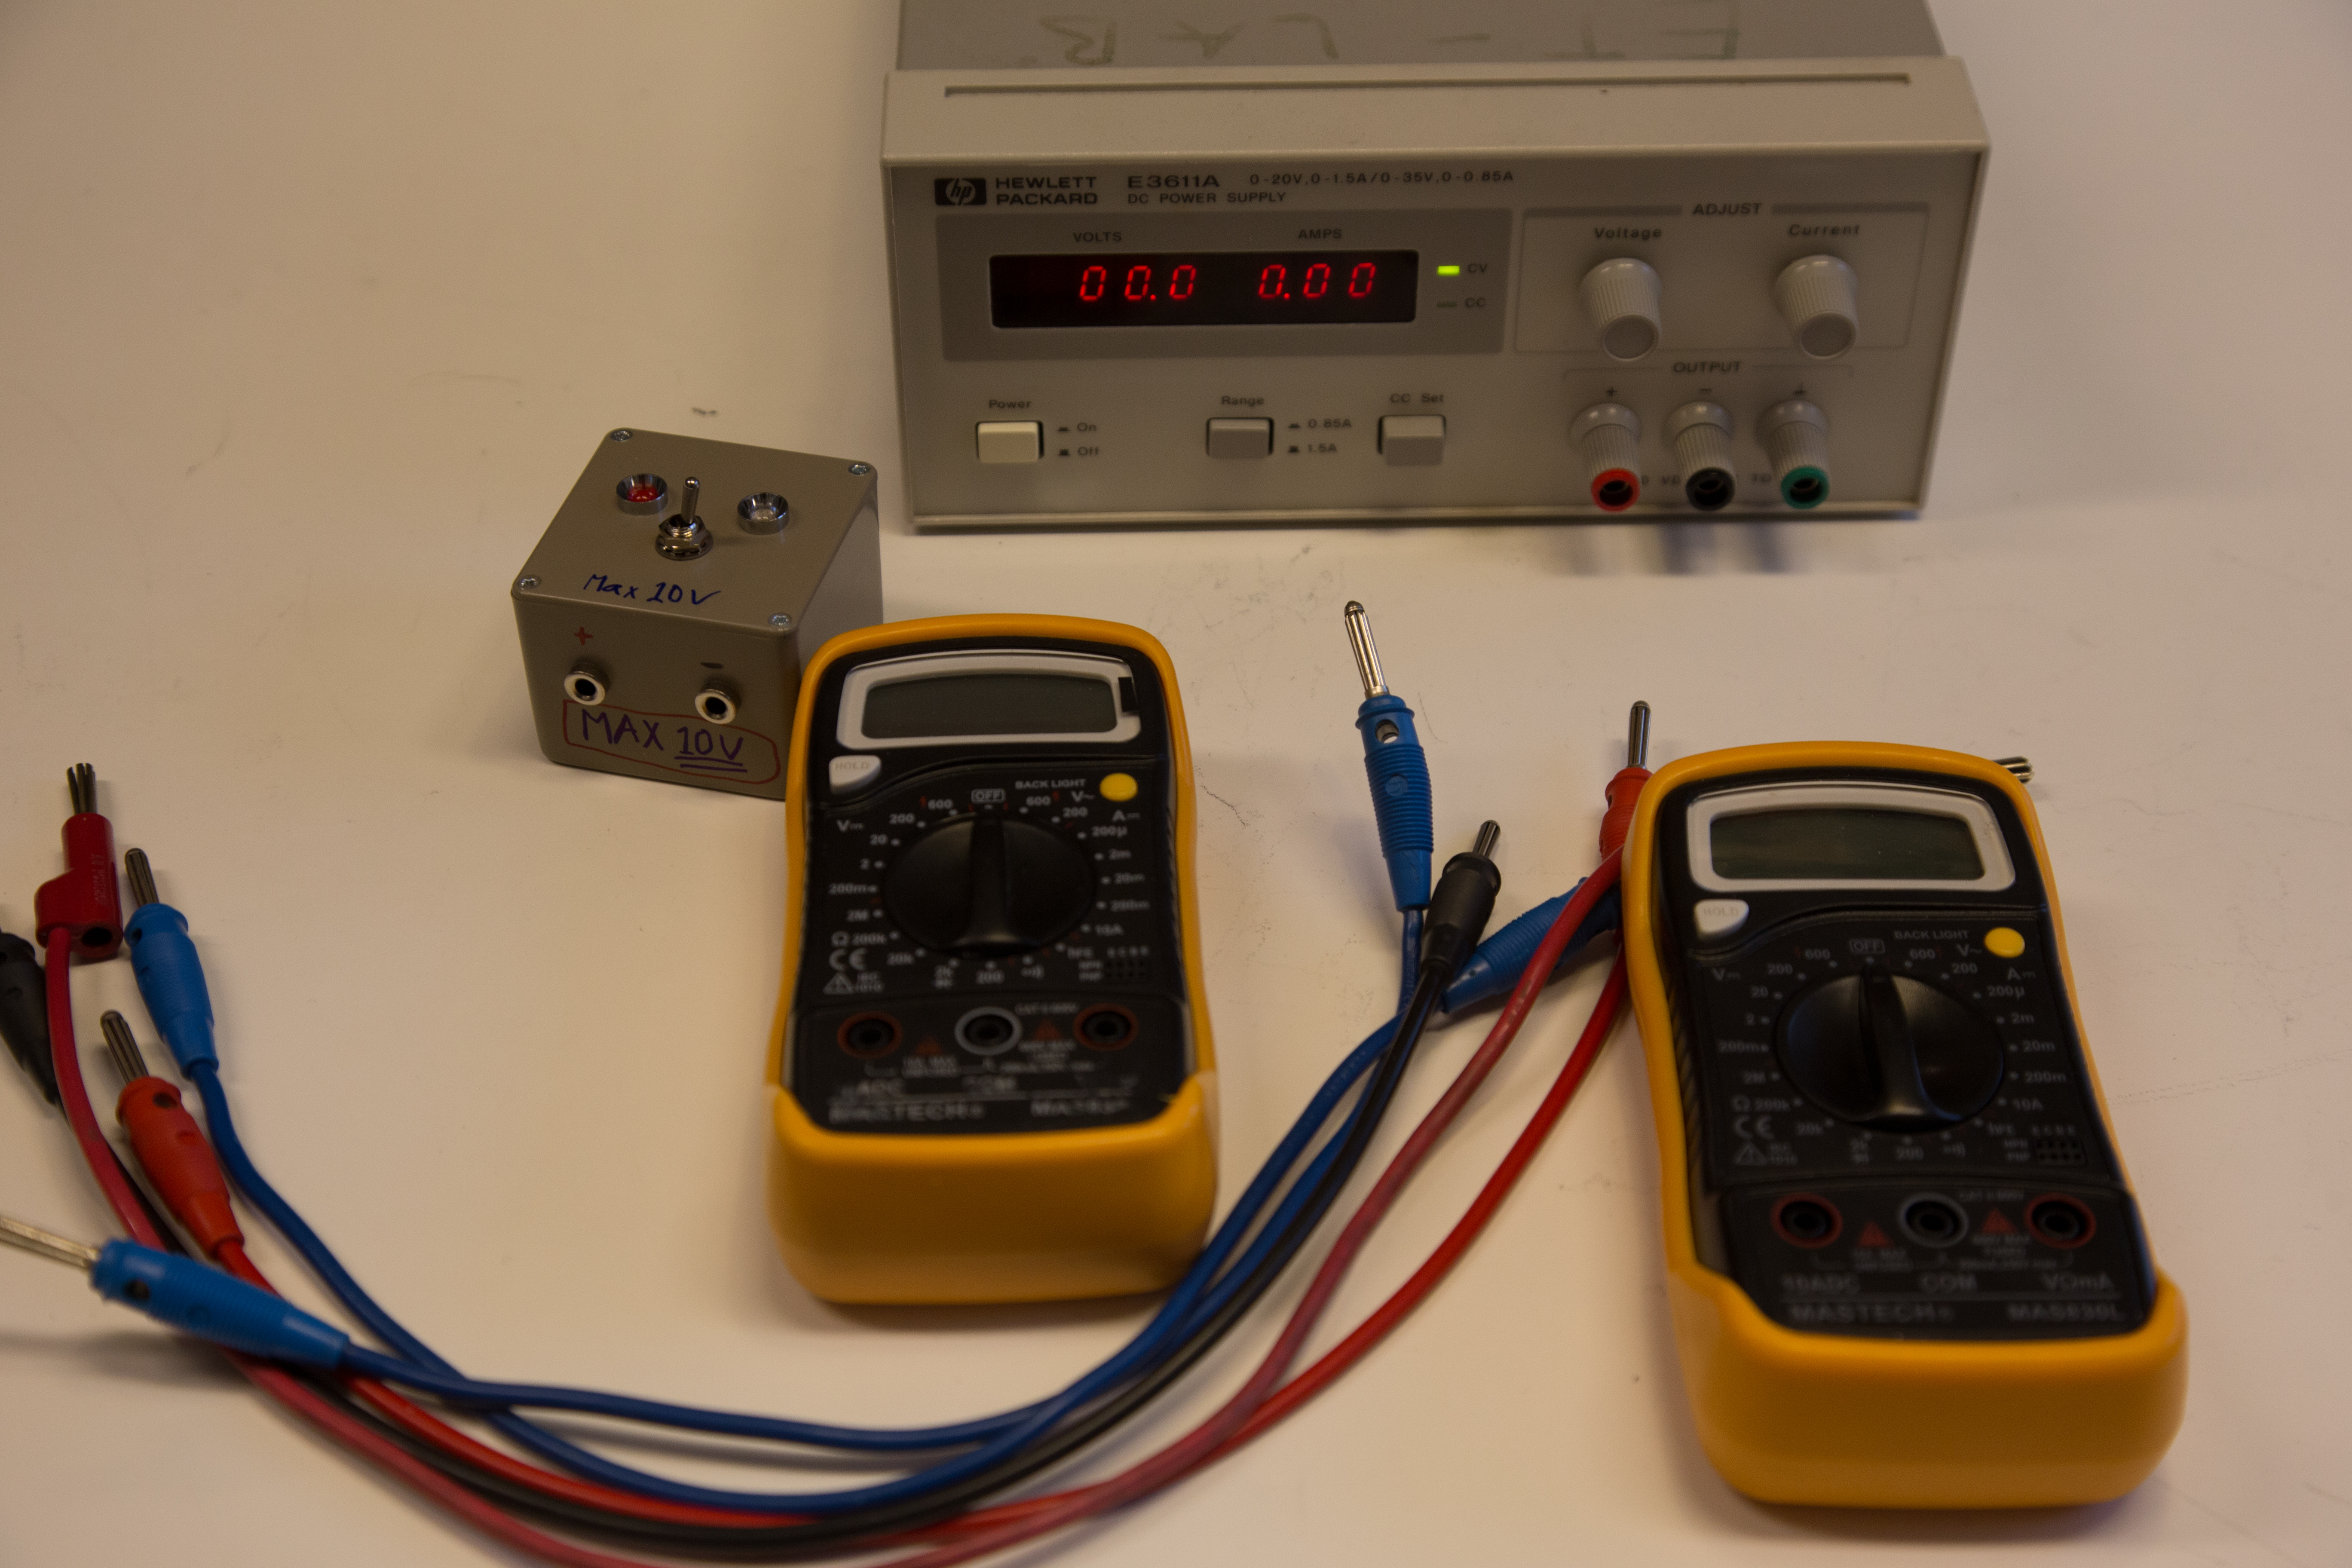
\includegraphics[width=1\textwidth]{../2015/IMG_3590.jpg}
}
%\caption{\label{figuren} Perioden $T$ som funktion av pendellängden.}
\end{figure}

\end{document}





%% På svenska ska citattecknet vara samma i både början och slut.
%% Använd två apostrofer (två enkelfjongar): ''.

%%För att referera till till tidigare fotnot:
%\footnotemark[\value{footnote}]

%% Inkludera PDF-dokument
%\includepdf[pages={1-}]{filnamn.pdf} %Filnamnet får INTE innehålla 'mellanslag'!

%% Figurer inkluderade som pdf-filer
%\begin{figure}\centering
%\centerline{ %centrerar även större bilder
%\includegraphics[width=1\textwidth]{filnamn.pdf}
%}
%\caption{\label{figuren} Perioden $T$ som funktion av pendellängden.}
%\end{figure}

%% Figurer inkluderade med xfigs "Combined PDF/LaTeX"
%\begin{figure}\centering
%\input{filnamn.pdf_t}
%\caption{\label{finafiguren} Perioden $T$ som funktion av
%  pendellängden.}
%\end{figure}


%% Figurer roterade 90 grader
%\begin{sidewaysfigure}\centering
%\centerline{ %centrerar även större bilder
%\includegraphics[width=1\textwidth]{filnamn.pdf}
%}
%\caption{\label{figuren} Perioden $T$ som funktion av pendellängden.}
%\end{sidewaysfigure}
